\documentclass{amsart}
\setlength{\oddsidemargin}{0.3in} \setlength{\evensidemargin}{0.3in} \setlength{\textwidth}{6.2in}

\usepackage{amsmath}
\usepackage{amsthm}
\usepackage{amsfonts}
\usepackage{amssymb}
\usepackage{amscd}
\usepackage{float}

% GRAPHICS--------------------------------------------------------
\usepackage{graphicx}
\graphicspath{ {C:/Users/Joseph/Pictures/581/} }

% THEOREMS -------------------------------------------------------
\theoremstyle{plain}
\newtheorem{thm}{Theorem}
\newtheorem{problem}{Problem}


% MATH -----------------------------------------------------------
\newcommand{\Q}{\ensuremath \mathbb{Q}}
\newcommand{\R}{\ensuremath \mathbb{R}}
\newcommand{\C}{\ensuremath \mathbb{C}}
\newcommand{\Z}{\ensuremath \mathbb{Z}}
\newcommand{\N}{\ensuremath \mathbb{N}}
\newcommand{\isom}{\ensuremath \cong}


\begin{document}
% This section gives the standard header to put on all of your homework, so you
% only need to change it to your section number, Homework number, and your name
\noindent {
\sc Econ 581 \hfill    % Change the '?' to your section number (2 for my class)
Solow Growth Model \hfill            % Change the '?' to the homework number (or, if you don't know that, fill in the due date)
Joe Cooprider                        % Change this to be your name
}

\bigskip
\begin{problem}
1.1.
\end{problem}
Below is for the first set of paramaters:\\
For $\tilde{k}_t$, the mean, standard deviation, coefficient of variation, relative coefficient of variation, correlation with Y, correlation with A, and autocorrelation are: 2.44142065,	0.016548655,	147.529857,	34.70249165,	0.008751021,	0.067324833,	0.977701483.\\
For $\tilde{y}_t$, the mean, standard deviation, coefficient of variation, relative coefficient of variation, correlation with Y, correlation with A, and autocorrelation are: 16.62386659,	3.910324347,	4.251275627,	1,	1,	-0.007854036,	0.023820669.
\\
For $\tilde{c}_t$, the mean, standard deviation, coefficient of variation, relative coefficient of variation, correlation with Y, correlation with A, and autocorrelation are: 15.79267326,	3.71480813,	4.251275627,	1,	1,	-0.007854036,	0.023820669.
\\
For $\tilde{i}_t$, the mean, standard deviation, coefficient of variation, relative coefficient of variation, correlation with Y, correlation with A, and autocorrelation are: 0.83119333,	0.195516217,	4.251275627,	1,	1,	-0.007854036,	0.023820669.\\
For $\tilde{A}_t$, the mean, standard deviation, coefficient of variation, relative coefficient of variation, correlation with Y, correlation with A, and autocorrelation are: 1.58956E+19,	8.99959E+19,	0.176625269,	0.041546417,	-0.007854036,	1,	0.996937289.\\
For $log(\tilde{k}_t)$, the mean, standard deviation, coefficient of variation, relative coefficient of variation, correlation with Y, correlation with A, and autocorrelation are: 0.387632637,	0.002943609	131.6862025,	11.68364577,	0.005119208,	0.069949226,	0.977701483
.\\
For $log(\tilde{y}_t)$, the mean, standard deviation, coefficient of variation, relative coefficient of variation, correlation with Y, correlation with A, and autocorrelation are: 1.20806748,	0.107183837,	11.27098554,	1,	1,	-0.002328091,	0.024272717.\\
For $log(\tilde{C}_t)$, the mean, standard deviation, coefficient of variation, relative coefficient of variation, correlation with Y, correlation with A, and autocorrelation are: 1.185791085,	0.107183837,	11.06315202,	0.981560306,	1,	-0.002328091,	0.024272717.\\
For $log(\tilde{I}_t)$, the mean, standard deviation, coefficient of variation, relative coefficient of variation, correlation with Y, correlation with A, and autocorrelation are: -0.092962515,	0.107183837,	-0.867318412,	-0.076951426,	1,	-0.002328091,	0.024272717.\\
For $\tilde{Z}_t$, the mean, standard deviation, coefficient of variation, relative coefficient of variation, correlation with Y, correlation with A, and autocorrelation are: -0.000227542,	0.077752194,	-0.002926504,	-0.000259649,	0.991863887,	-0.001159019,	0.018696135.\\ \\
For the second set of paramaters:\\
For $\tilde{k}_t$, the mean, standard deviation, coefficient of variation, relative coefficient of variation, correlation with Y, correlation with A, and autocorrelation are: 19.33021123,	0.149250979,	129.5148037,	30.47115415,	0.038584394,	-0.044818267,	0.982903312.\\
For $\tilde{y}_t$, the mean, standard deviation, coefficient of variation, relative coefficient of variation, correlation with Y, correlation with A, and autocorrelation are: 32.90138658,	7.740761623,	4.250406896,	1,	1,	-0.029745081,	0.025466048.
\\
For $\tilde{c}_t$, the mean, standard deviation, coefficient of variation, relative coefficient of variation, correlation with Y, correlation with A, and autocorrelation are: 26.32110927,	6.192609298,	4.250406896,	1,	1,	-0.029745081,	0.025466048.
\\
For $\tilde{i}_t$, the mean, standard deviation, coefficient of variation, relative coefficient of variation, correlation with Y, correlation with A, and autocorrelation are: 6.580277316,	1.548152325,	4.250406896,	1,	1,	-0.029745081,	0.025466048.\\
For $\tilde{A}_t$, the mean, standard deviation, coefficient of variation, relative coefficient of variation, correlation with Y, correlation with A, and autocorrelation are: 6.62065E+19,	2.14821E+20,	0.308193504,	0.072509176,	-0.029745081,	1,	0.996919013.\\
For $log(\tilde{k}_t)$, the mean, standard deviation, coefficient of variation, relative coefficient of variation, correlation with Y, correlation with A, and autocorrelation are: 1.286636314,	0.003312455,	388.4238386,	27.63552714,	0.034335448,	-0.170332691,	0.982366333.\\
For $log(\tilde{y}_t)$, the mean, standard deviation, coefficient of variation, relative coefficient of variation, correlation with Y, correlation with A, and autocorrelation are: 1.506063174,	0.108410611,	13.89221185,	1,	1,	0.010024524,	0.023028172.\\
For $log(\tilde{C}_t)$, the mean, standard deviation, coefficient of variation, relative coefficient of variation, correlation with Y, correlation with A, and autocorrelation are: 1.409153161,	0.108410611,	12.99829554,	0.935653421,	1,	0.010024524,	0.023028172.\\
For $log(\tilde{I}_t)$, the mean, standard deviation, coefficient of variation, relative coefficient of variation, correlation with Y, correlation with A, and autocorrelation are: 0.806622141,	0.107129336,	7.529423524,	0.535750763,	1,	-0.016170752,	0.032461931.\\
For $\tilde{Z}_t$, the mean, standard deviation, coefficient of variation, relative coefficient of variation, correlation with Y, correlation with A, and autocorrelation are: 0.000381011,	0.077803028,	0.004897117,	0.000348451,	0.991578612,	-0.01440627,	0.030289601.\\ \\

For the third set of paramaters:\\
For $\tilde{k}_t$, the mean, standard deviation, coefficient of variation, relative coefficient of variation, correlation with Y, correlation with A, and autocorrelation are: 2.44154615,	0.018281284,	133.5544155,	31.46094187,	0.030572945,	0.009737369,	0.981720227.\\
For $\tilde{y}_t$, the mean, standard deviation, coefficient of variation, relative coefficient of variation, correlation with Y, correlation with A, and autocorrelation are: 16.62615487,	3.91656457,	4.245086369,	1,	1,	-0.017171241,	0.032961885.
\\
For $\tilde{c}_t$, the mean, standard deviation, coefficient of variation, relative coefficient of variation, correlation with Y, correlation with A, and autocorrelation are: 15.79484713,	3.720736342,	4.245086369,	1,	1,	-0.017171241,	0.032961885.
\\
For $\tilde{i}_t$, the mean, standard deviation, coefficient of variation, relative coefficient of variation, correlation with Y, correlation with A, and autocorrelation are: 0.831307744,	0.195828229,	4.245086369,	1,	1,	-0.017171241,	0.032961885.\\
For $\tilde{A}_t$, the mean, standard deviation, coefficient of variation, relative coefficient of variation, correlation with Y, correlation with A, and autocorrelation are: 3.99127E+19,	1.82093E+20,	0.219188954,	0.051633568,	-0.017171241,	1,	0.996454884.\\
For $log(\tilde{k}_t)$, the mean, standard deviation, coefficient of variation, relative coefficient of variation, correlation with Y, correlation with A, and autocorrelation are: 0.387652754,	0.003253728,	119.1410971,	10.60446978,	0.031172048,	0.028851351,	0.981720227.\\
For $log(\tilde{y}_t)$, the mean, standard deviation, coefficient of variation, relative coefficient of variation, correlation with Y, correlation with A, and autocorrelation are: 1.208067305,	0.107527239,	11.2349886,	1,	1,	-0.004345455,	0.031840109.\\
For $log(\tilde{C}_t)$, the mean, standard deviation, coefficient of variation, relative coefficient of variation, correlation with Y, correlation with A, and autocorrelation are: 1.18579091,	0.107527239,	11.02781881,	0.981560303,	1,	-0.004345455,	0.031840109.\\
For $log(\tilde{I}_t)$, the mean, standard deviation, coefficient of variation, relative coefficient of variation, correlation with Y, correlation with A, and autocorrelation are: -0.092086473,	0.107459799,	-0.856938823,	-0.07617103,	1,	0.015610874,	0.034508809.\\
For $\tilde{Z}_t$, the mean, standard deviation, coefficient of variation, relative coefficient of variation, correlation with Y, correlation with A, and autocorrelation are: 0.000561621,	0.077553116,	0.007241762,	0.000637963,	0.992130811,	0.010751721,	0.020834155.\\
\begin{problem}
1.b.
\end{problem}

\begin{figure}[H]
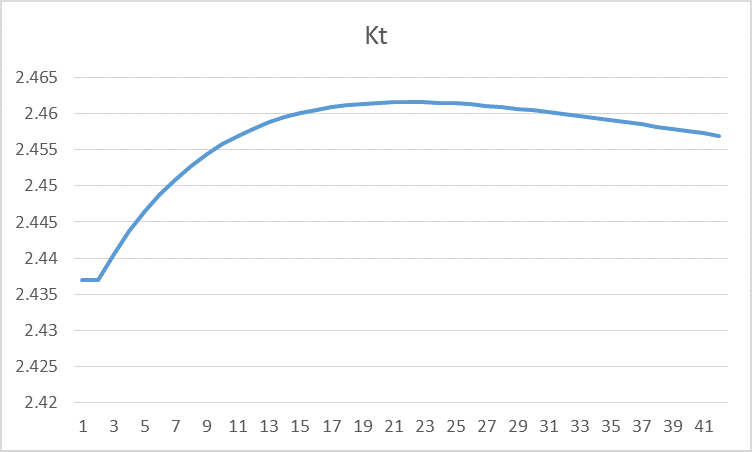
\includegraphics[scale=.50]{12a.png}
\end{figure}
\begin{figure}[H]
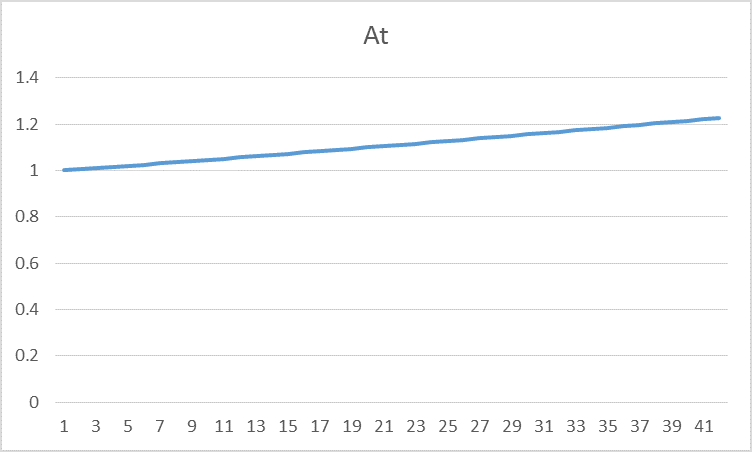
\includegraphics[scale=.50]{12b.png}
\end{figure}
\begin{figure}[H]
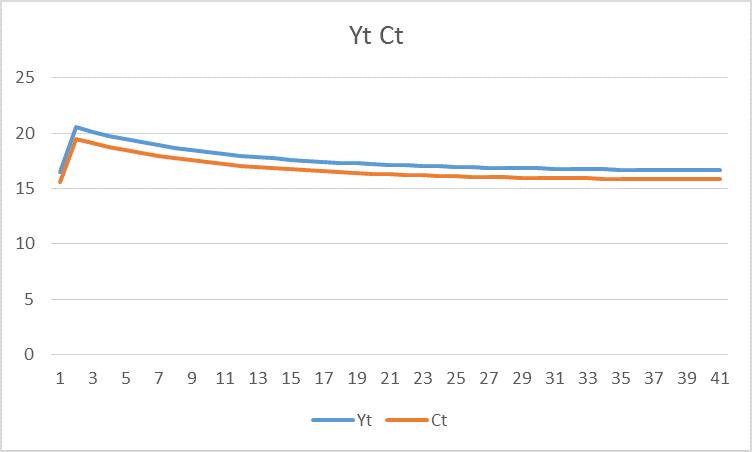
\includegraphics[scale=.50]{12c.png}
\end{figure}
\begin{figure}[H]
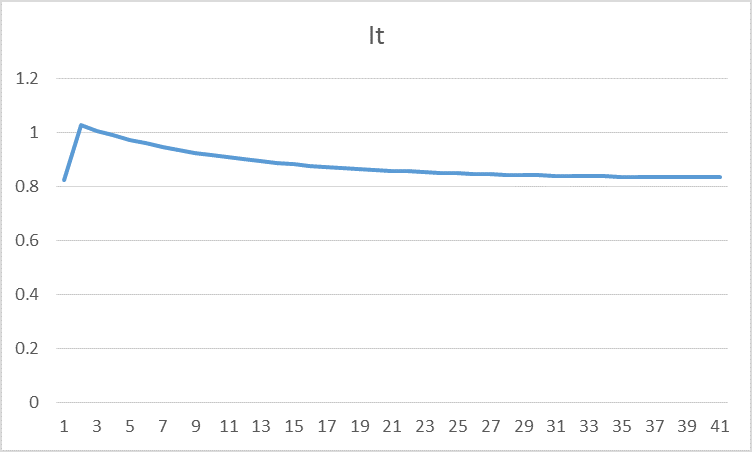
\includegraphics[scale=.50]{12d.png}
\end{figure}
\begin{figure}[H]
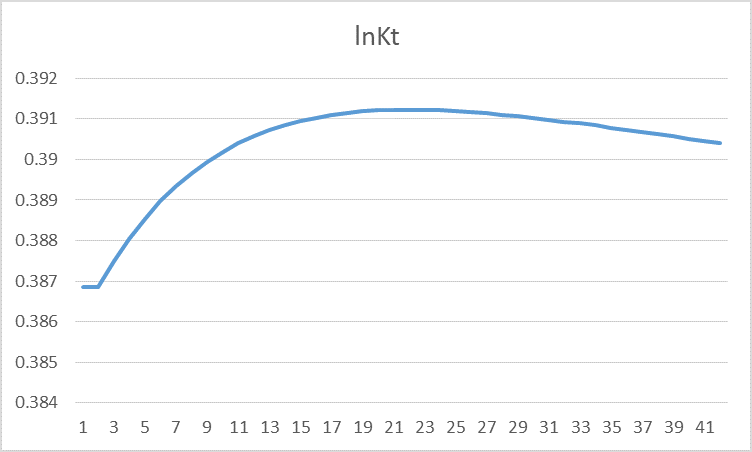
\includegraphics[scale=.50]{12e.png}
\end{figure}
\begin{figure}[H]
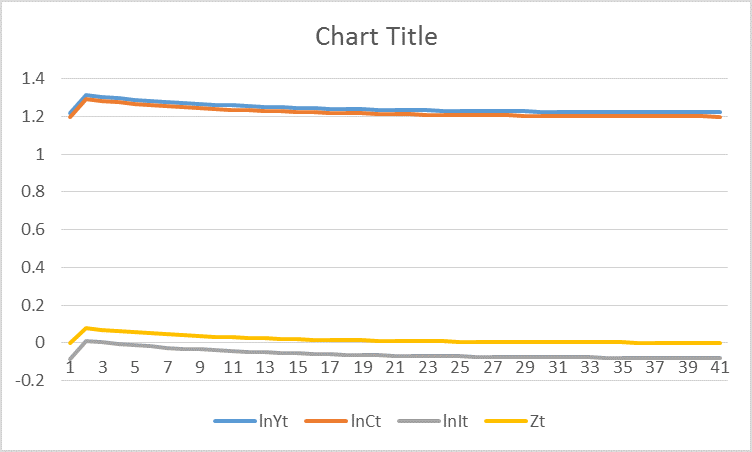
\includegraphics[scale=.50]{12f.png}
\end{figure}

\begin{problem}
1.c.
\end{problem}
For the first set of paramaters:
For $\tilde{k}_t$, the mean, standard deviation, coefficient of variation, relative coefficient of variation, correlation with Y, correlation with A, and autocorrelation are: 2.436367142,	0.003270556,	744.9396976,	22.2741009,	0.999083849,	0.120164945,	0.999897094.\\
For $\tilde{y}_t$, the mean, standard deviation, coefficient of variation, relative coefficient of variation, correlation with Y, correlation with A, and autocorrelation are: 16.44194142,	0.491622964,	33.44420952,	1,	1,	0.811330798,	0.999862829.
\\
For $\tilde{c}_t$, the mean, standard deviation, coefficient of variation, relative coefficient of variation, correlation with Y, correlation with A, and autocorrelation are: 15.61984435,	0.467041816,	33.44420952,	1,	1,	0.811330798,	0.999862829.
\\
For $\tilde{i}_t$, the mean, standard deviation, coefficient of variation, relative coefficient of variation, correlation with Y, correlation with A, and autocorrelation are: 0.822097071,	0.024581148,	33.44420952,	1,	1,	0.811330798,	0.999862829.\\
For $\tilde{A}_t$, the mean, standard deviation, coefficient of variation, relative coefficient of variation, correlation with Y, correlation with A, and autocorrelation are: 0.999745803,	0.001699629,	588.2142476,	17.58792497,	0.811330798,	1,	0.989321611.\\
For $log(\tilde{k}_t)$, the mean, standard deviation, coefficient of variation, relative coefficient of variation, correlation with Y, correlation with A, and autocorrelation are: 10.30626613,	6.886540103,	1.496581154,	0.000718038,	0.12033207,	0.097343628,	0.999987972.\\
For $log(\tilde{y}_t)$, the mean, standard deviation, coefficient of variation, relative coefficient of variation, correlation with Y, correlation with A, and autocorrelation are: 1.216082417,	0.000583459,	2084.265232,	1,	1,	0.81132256,	0.999862841.\\
For $log(\tilde{C}_t)$, the mean, standard deviation, coefficient of variation, relative coefficient of variation, correlation with Y, correlation with A, and autocorrelation are: 1.193806022	0.000583459,	2046.085324,	0.981681838,	1,	0.81132256,	0.999862841.\\
For $log(\tilde{I}_t)$, the mean, standard deviation, coefficient of variation, relative coefficient of variation, correlation with Y, correlation with A, and autocorrelation are: -0.084947579	0.000583459,	-145.5931623,	-0.069853472,	1,	0.81132256,	0.999862841.\\
For $\tilde{Z}_t$, the mean, standard deviation, coefficient of variation, relative coefficient of variation, correlation with Y, correlation with A, and autocorrelation are: all zeros.\\

\begin{figure}[H]
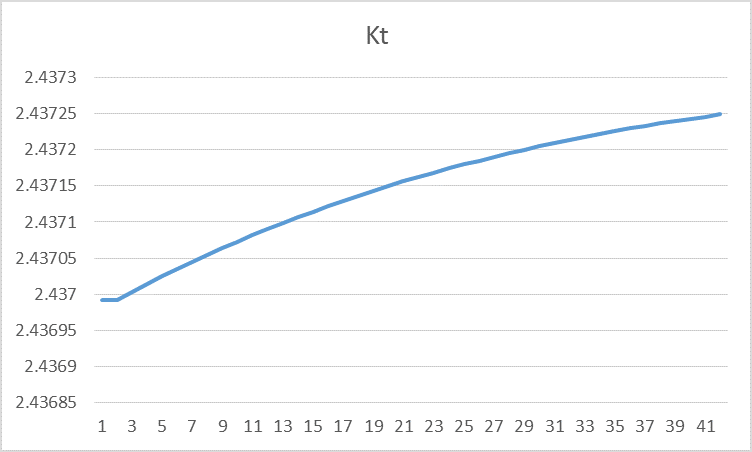
\includegraphics[scale=.50]{13a.png}
\end{figure}
\begin{figure}[H]
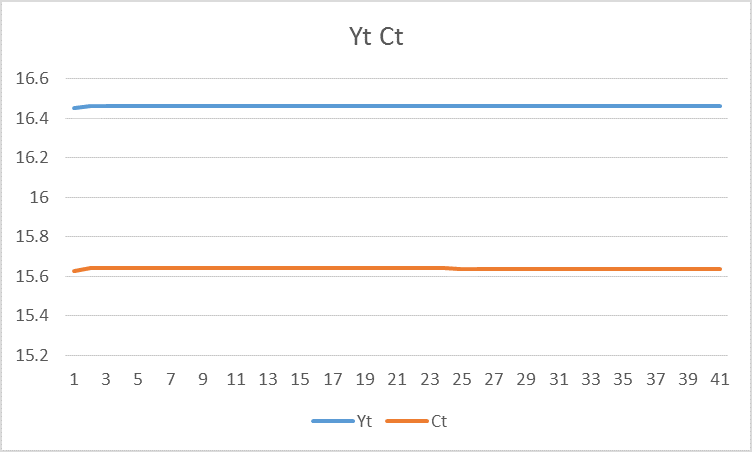
\includegraphics[scale=.50]{13b.png}
\end{figure}
\begin{figure}[H]
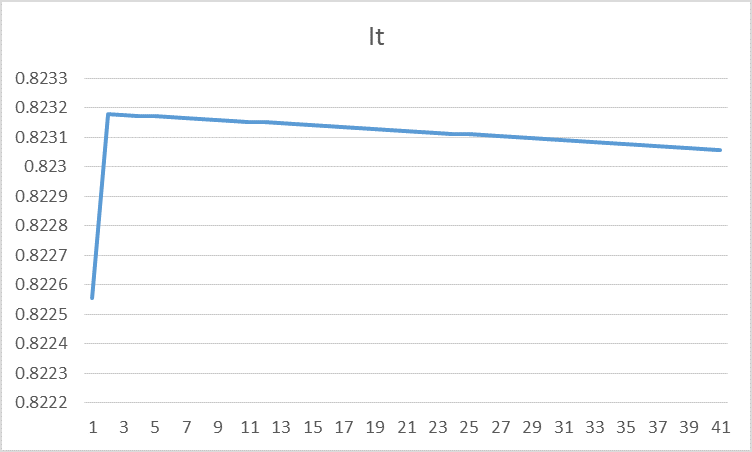
\includegraphics[scale=.50]{13c.png}
\end{figure}
\begin{figure}[H]
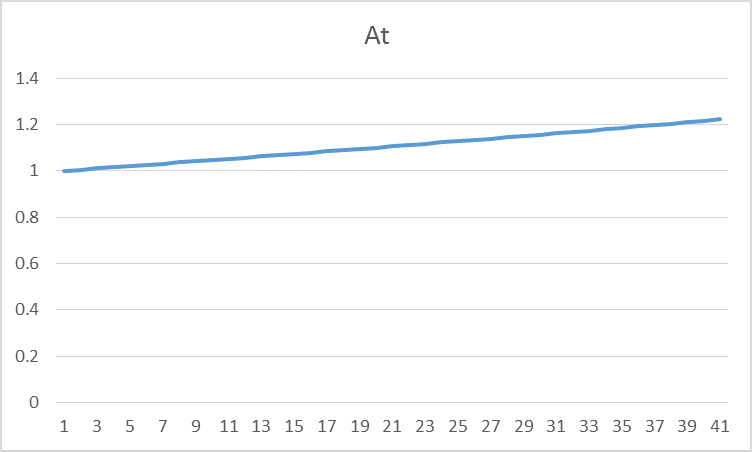
\includegraphics[scale=.50]{13d.png}
\end{figure}
\begin{figure}[H]
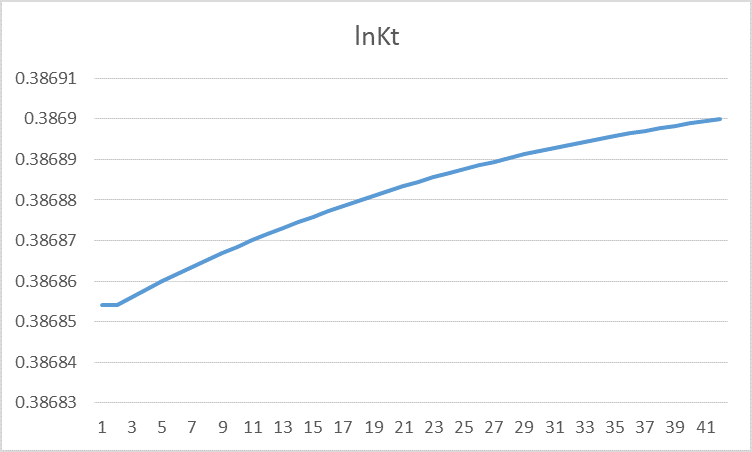
\includegraphics[scale=.50]{13e.png}
\end{figure}
\begin{figure}[H]
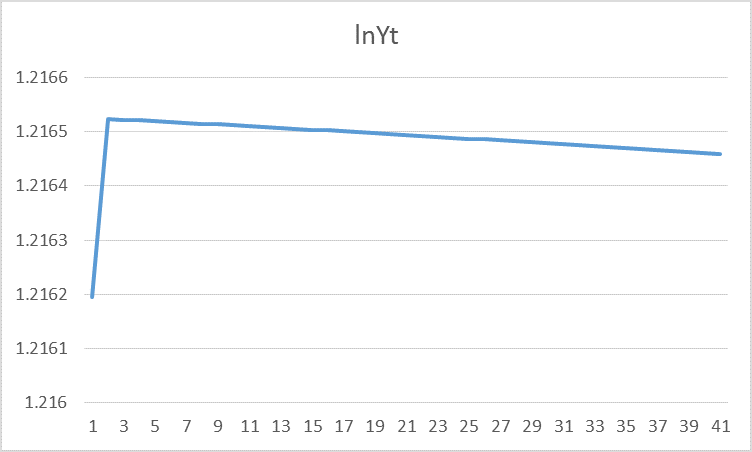
\includegraphics[scale=.50]{13f.png}
\end{figure}
\begin{figure}[H]
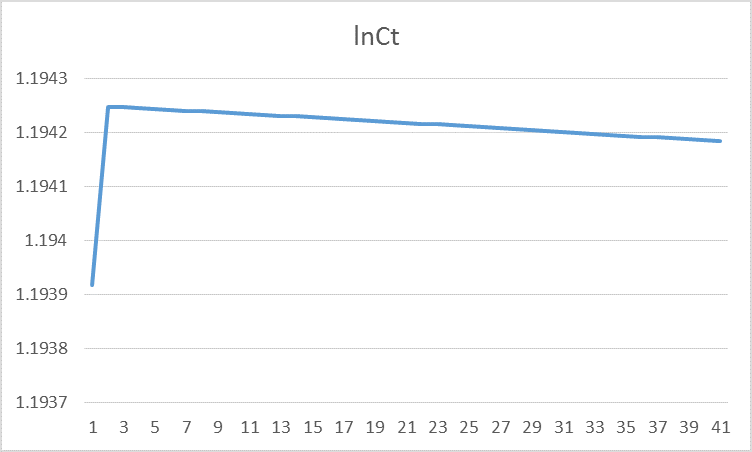
\includegraphics[scale=.50]{13g.png}
\end{figure}
\begin{figure}[H]
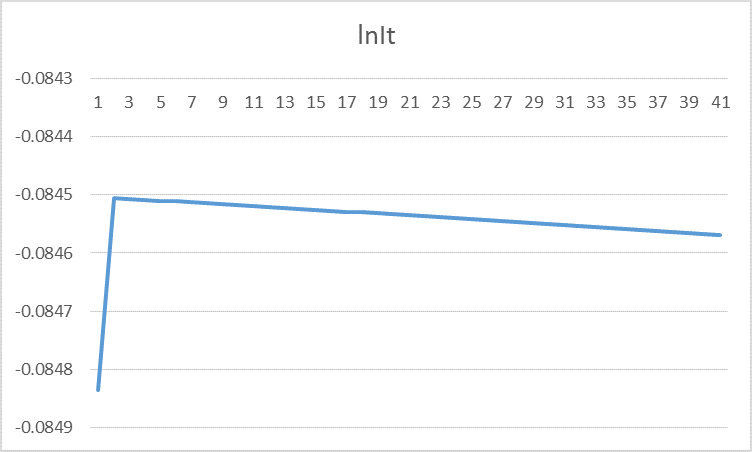
\includegraphics[scale=.50]{13h.png}
\end{figure}
\begin{figure}[H]
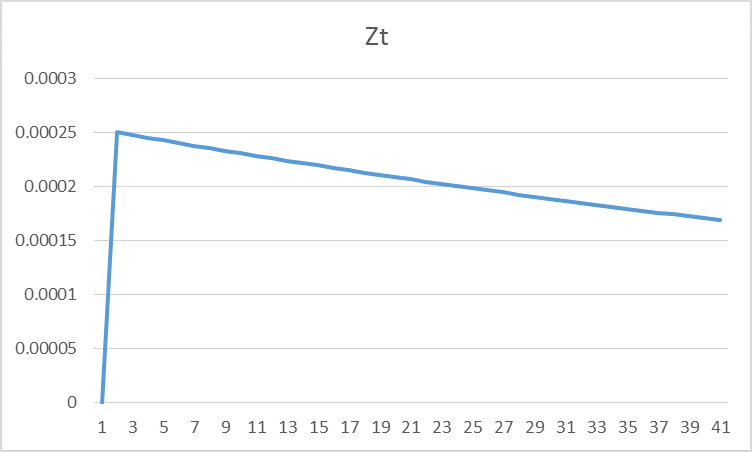
\includegraphics[scale=.50]{13i.png}
\end{figure}

For the second set of paramaters:
For $\tilde{k}_t$, the mean, standard deviation, coefficient of variation, relative coefficient of variation, correlation with Y, correlation with A, and autocorrelation are: 2.444678672,	0.020320086,	120.3084803,	28.79617487,	0.045494757,	-0.112648907,	0.984864362.\\
For $\tilde{y}_t$, the mean, standard deviation, coefficient of variation, relative coefficient of variation, correlation with Y, correlation with A, and autocorrelation are: 16.73062081,	4.004521389,	4.177932687,	1,	1,	0.023766636,	0.044093365.
\\
For $\tilde{c}_t$, the mean, standard deviation, coefficient of variation, relative coefficient of variation, correlation with Y, correlation with A, and autocorrelation are: 15.89408977,	3.804295319,	4.177932687,	1,	1,	0.023766636,	0.044093365.
\\
For $\tilde{i}_t$, the mean, standard deviation, coefficient of variation, relative coefficient of variation, correlation with Y, correlation with A, and autocorrelation are:0.83653104,	0.200226069,	4.177932687,	1,	1,	0.023766636,	0.044093365.\\
For $\tilde{A}_t$, the mean, standard deviation, coefficient of variation, relative coefficient of variation, correlation with Y, correlation with A, and autocorrelation are: 0.999579122,	0.001868439,	534.9807613,	128.0491576,	0.023766636,	1,	0.990940538.\\
For $log(\tilde{k}_t)$, the mean, standard deviation, coefficient of variation, relative coefficient of variation, correlation with Y, correlation with A, and autocorrelation are: 15.07415464,	8.296185049,	1.816998361,	0.161859889,	-0.013069733,	-0.214748505,	0.999991542.\\
For $log(\tilde{y}_t)$, the mean, standard deviation, coefficient of variation, relative coefficient of variation, correlation with Y, correlation with A, and autocorrelation are: 1.210794062,	0.107858651,	11.22574823,	1,	1,	0.022987192,	0.045019853.\\
For $log(\tilde{C}_t)$, the mean, standard deviation, coefficient of variation, relative coefficient of variation, correlation with Y, correlation with A, and autocorrelation are: 1.188517667	0.107858651,	11.01921501,	0.98160183,	1,	0.022987192,	0.045019853.\\
For $log(\tilde{I}_t)$, the mean, standard deviation, coefficient of variation, relative coefficient of variation, correlation with Y, correlation with A, and autocorrelation are: -0.090235934,	0.107858651,	-0.836612851,	-0.074526244,	1,	0.022987192,	0.045019853.\\
For $\tilde{Z}_t$, the mean, standard deviation, coefficient of variation, relative coefficient of variation, correlation with Y, correlation with A, and autocorrelation are: 0.001499222	0.078560334,	0.019083703,	0.001699479,	0.991588202,	-0.011609685,	0.037249566.\\


\end{document}